% $Id: Note_ResFit_QCDMC.tex,v 1.4 2010/07/13 17:26:14 mschrode Exp $


\section{Study with a QCD Monte Carlo Simulation}\label{sec:ResFit:QCDMC}

The maximum likelihood method is also tested on a sample of simulated QCD multijet events in $pp$ collisions at 7\tev centre-of-mass energy.
They have been generated with PYTHIA and processed through the full CMS detector simulation application based on GEANT4\footnote{The used data set is \texttt{/QCDFlat\_Pt15to3000/Spring10-START3X\_V26\_S09-v1/GEN-SIM-RECO}}.
The events are weighted corresponding to an integrated luminosity of 50\pbinv.


\subsection{Event selection}\label{sec:ResFit:QCDMC:EvtSel}

Jets are reconstructed from calorimeter towers using the anti-$k_{T}$ jet clustering algorithm~\cite{bib:akj} with parameter size $d=0.5$.
Jet energy corrections~\cite{bib:cmspas:jec} are applied to remove the $\eta$ and \pt dependence of the jet energy scale.
Dijet events are selected in the following way:
\begin{enumerate}
\item The third jet is required to have small \pt compared to the leading two jets by imposing \mbox{$\ptrel < x$}, with \mbox{$\ptrel = \frac{2\pti{3}}{\pti{1} + \pti{2}}$}, in order to ensure a dijet topology.
  The value of $x$ is varied in course of the analysis as discussed in Section~\ref{sec:ResFit:QCDMC:AddJetAct}.
\item Both leading jets are required to be in the same pseudorapidity bin, which are defined in Table~\ref{tab:ResFit:QCDMC:MCTruthReso}.
  This accounts for the dependence of the jet \pt response on $\eta$ due to
  \begin{itemize}
  \item different calorimeter geometries and material budgets in front of the calorimeters in different pseudorapidity regions;
  \item the fact that the intrinsic calorimeter resolution is energy rather than \pt dependent.
  \end{itemize}
\item In order to reject jets clustered from noise in the hadronic calorimeter component, the fraction $f_{\text{em}}$ of energy deposited in the electromagnetic component is required to be \mbox{$f_{\text{em}} > 0.01$} for both leading jets~\cite{bib:cmspas:jetid}.
\end{enumerate}
The jet \ptparticle spectrum of the leading two jets after the dijet selection above is shown in Figure~\ref{fig:ResFit:QCDMC:MCTruthReso} (\textit{left}).


\subsection{Gaussian resolution from Monte Carlo truth information}\label{sec:ResFit:QCDMC:MCTruthReso}

The jet \pt resolution is determined from Monte Carlo truth information, first, as a reference to compare the measured resolution to, and second, as an input $r_{0}$ in~\eqref{eq:ResFit:Method:ModifiedSpectrum} to incorporate the the selection bias into the dijet likelihood (comp. Section~\ref{sec:ResFit:Method:Biases}).
\begin{figure}[ht]
  \centering
  \begin{tabular}{cc}
    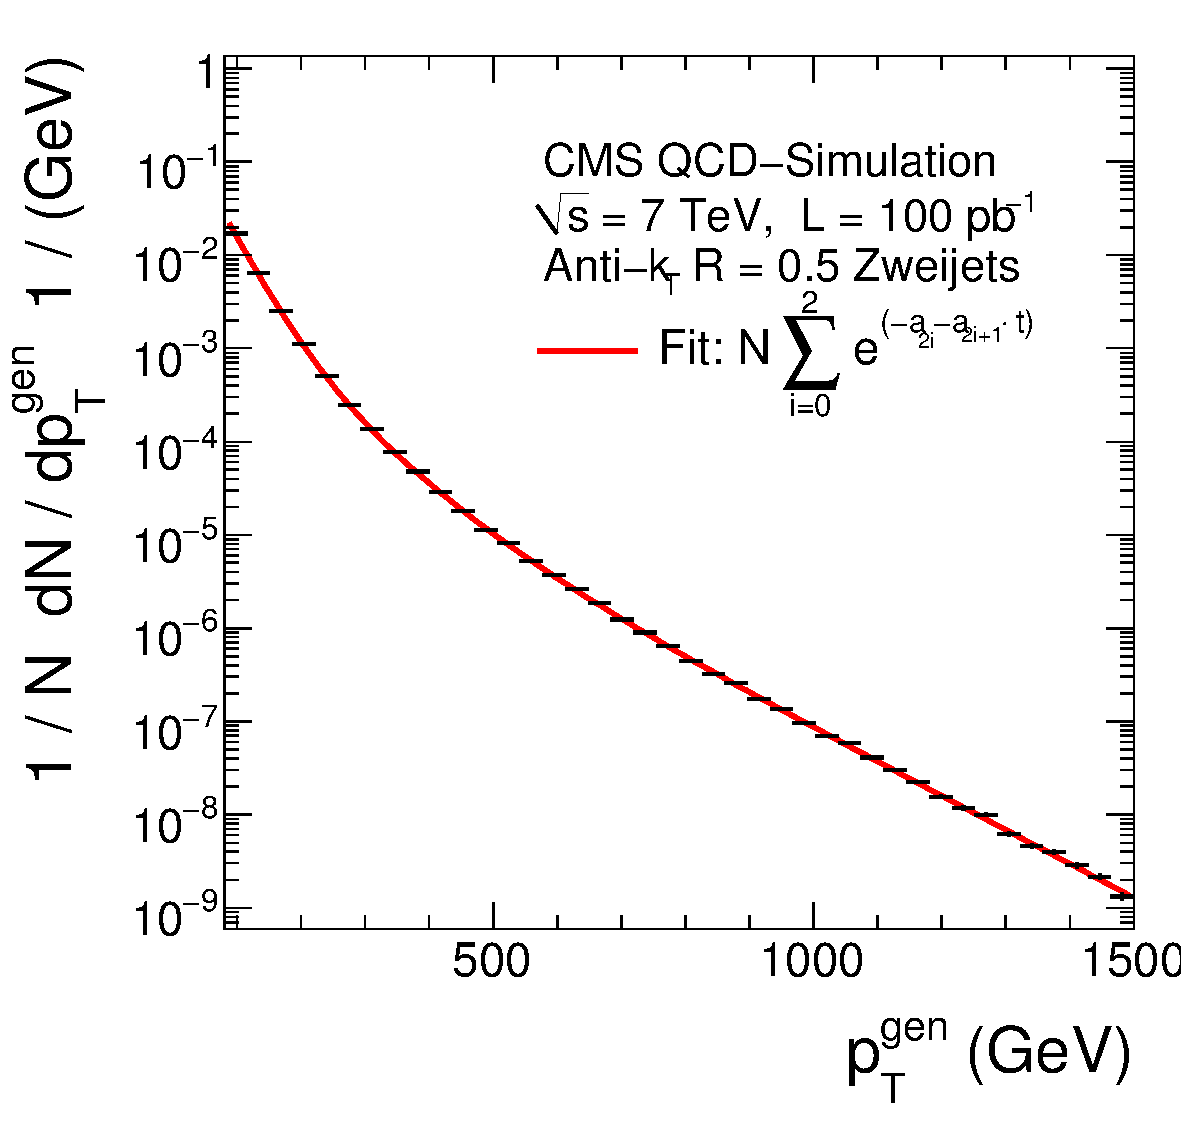
\includegraphics[width=0.45\textwidth]{figures/resFit_QCD_MCSpectrum}
    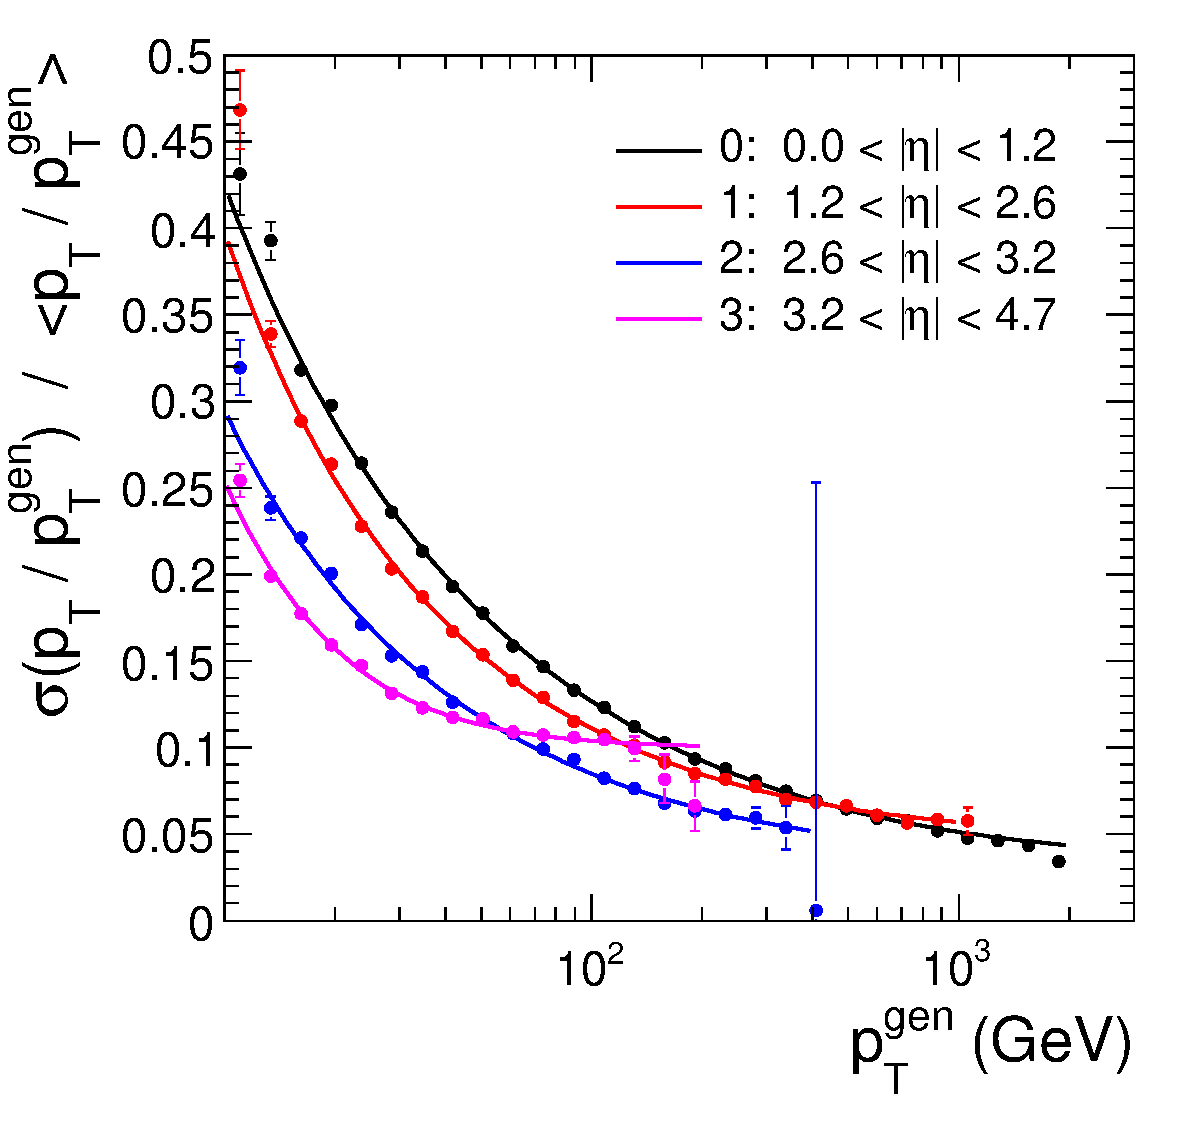
\includegraphics[width=0.45\textwidth]{figures/resFit_QCD_MCTruthResolution}
  \end{tabular}
  \caption{(\textit{Left}) QCD dijet \ptparticle spectrum. (\textit{Right}) Relative Gaussian jet \pt resolution $\sigma/\pt$ derived from Monte Carlo truth as a function of \pt in different $\eta$ bins.}
  \label{fig:ResFit:QCDMC:MCTruthReso}
\end{figure}
The determination follows closely~\cite{bib:cmsan:mcjer}:
In each event, the two jets with highest particle level jet \pt, \ptparticle, are selected and the response distributions \mbox{$\ptmeas / \ptparticle$} are recorded in different bins of \ptparticle and $\eta$ (the $\eta$ binning is listed in Table~\ref{tab:ResFit:QCDMC:MCTruthReso}).

--- Define matching ??? ---

The central part of each distribution --- defined by the interval of 1.5 standard deviations around the mean --- is fitted with a Gaussian.
In each $\eta$ bin, the fitted Gaussian widths $\sigma$ are interpolated for different \pt by the usual parametrisation function~\eqref{eq:ResFit:ToyMC:Sigma}.
The fitted Gaussian widths and the interpolation functions are shown in Fig.~\ref{fig:ResFit:QCDMC:MCTruthReso}; the corresponding parameter values are listed in Table~\ref{tab:ResFit:QCDMC:MCTruthReso}.
\begin{table}[ht]
  \caption{Parameters of the MC truth resolution $\sigma$.}
  \centering
  \begin{tabular}[h]{cccccc}
    \toprule
    & $|\eta_{\text{min}}|$ & $|\eta_{\text{max}}|$ & $\xi_{0}\,(\text{Ge}\kern-0.06667em\text{V})$ & $\xi_{1}\,(\sqrt{\text{Ge}\kern-0.06667em\text{V}})$ & $\xi_{2}$ \\
    \midrule
    $0$ & $0$ & $1.2$ & $1.9\pm0.2$ & $1.205\pm0.006$  & $0.0342\pm0.0007$ \\
    $1$ & $1.2$ & $2.6$ & $2.51\pm0.09$ & $0.968\pm0.009$  & $0.0483\pm0.0009$ \\
    $2$ & $2.6$ & $3.2$ & $1.7\pm0.18$ & $0.76\pm0.02$  & $0.035\pm0.004$ \\
    $3$ & $3.2$ & $4.7$ & $2.2\pm0.1$ & $0.2\pm0.1$  & $0.099\pm0.003$ \\
    \bottomrule
  \end{tabular}
  \label{tab:ResFit:QCDMC:MCTruthReso}
\end{table}




\subsection{Effects from additional jet activity}\label{sec:ResFit:QCDMC:AddJetAct}

One assumption of the maximum likelihood method is the \pt balance on
particle level of the two leading jets in each dijet event.
In realistic QCD events, however, additional jets, e.g. from hard
gluon radiation, cause a \ptparticle imbalance.
The resolution measurement, therefore, will be biased
towards larger values.
The effect is demonstrated in Fig.~\ref{fig:ResFit:QCDMC:AddJetAct:Fit}: 
The Gaussian resolution $\sigma$ ~\eqref{eq:ResFit:ToyMC:Sigma} is derived using the maximum
likelihood fit.
As expected, the result does not agree with the Monte Carlo truth
resolution.
\begin{figure}[ht]
  \centering
  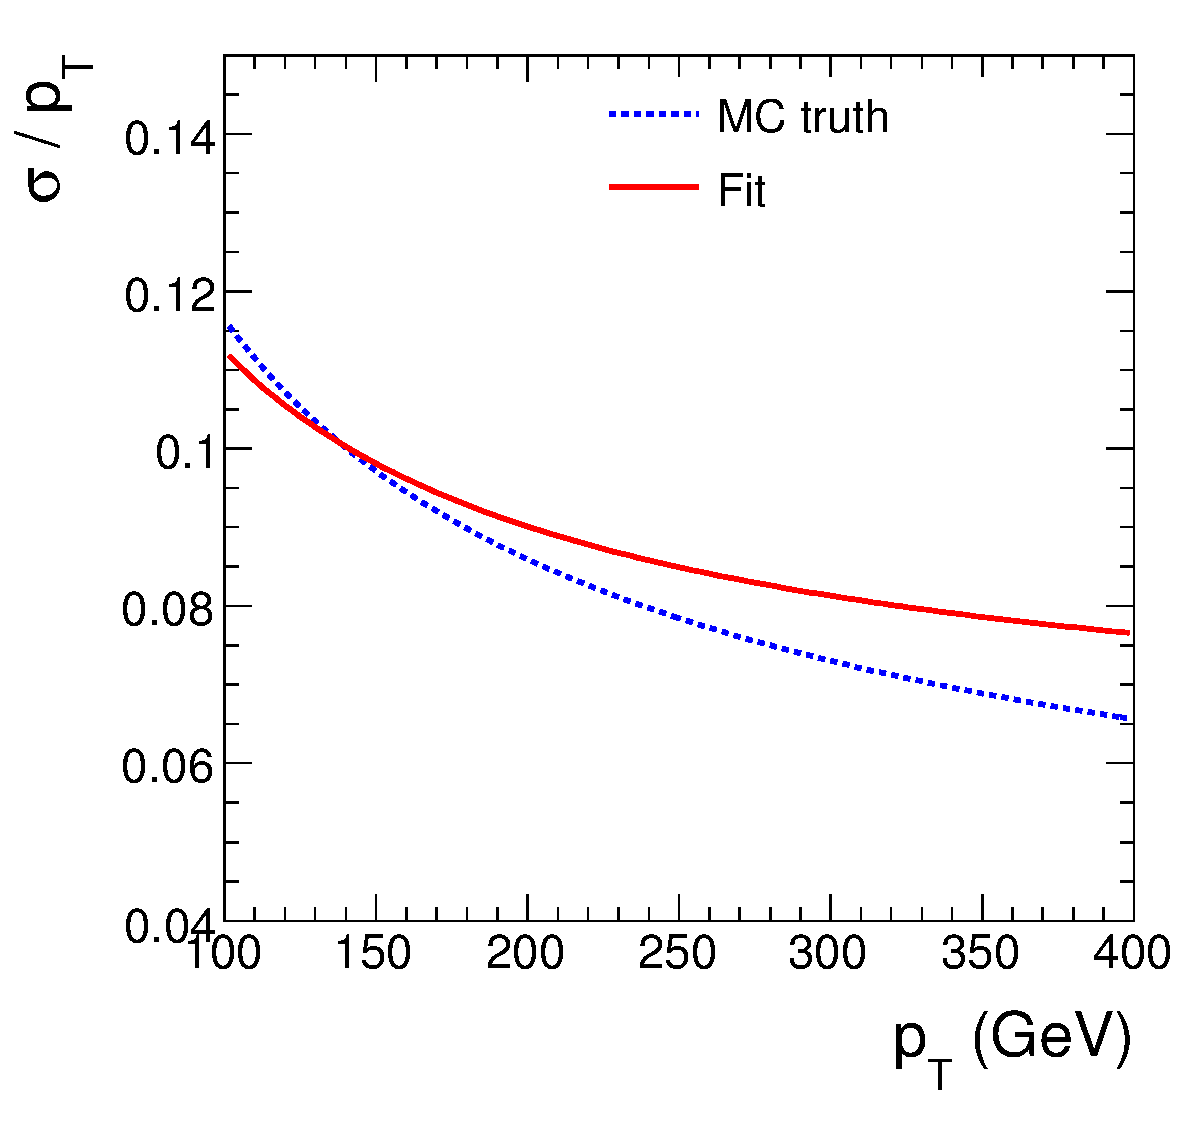
\includegraphics[width=0.45\textwidth]{figures/resFit_PtDependentSigma}
  \caption{Bias due to additional jet activity: \pt dependent $\sigma$}
  \label{fig:ResFit:QCDMC:AddJetAct:Fit}
\end{figure}

In the following Section~\ref{sec:ResFit:QCDMC:Extrapolation}, a method is proposed to correct the resolution
measurement for the effects of additional jet activity.
